\documentclass[10pt]{article}

\usepackage[margin=0.75in]{geometry}
\usepackage{amsmath, amssymb}
\usepackage{graphicx}
\usepackage[T1]{fontenc}
\usepackage{inconsolata}
\usepackage{titlesec}
\usepackage{fancyhdr}
\usepackage{microtype}

\graphicspath{{../}}

\setlength{\parindent}{0pt}
\setlength{\parskip}{4pt}
\renewcommand{\baselinestretch}{1.05}

\titleformat{\section}{\ttfamily\normalsize\bfseries\MakeUppercase}{\thesection}{0.6em}{}
\titlespacing*{\section}{0pt}{8pt}{2pt}
\titleformat{\subsection}{\ttfamily\small\MakeUppercase}{\thesubsection}{0.6em}{}
\titlespacing*{\subsection}{0pt}{6pt}{2pt}

\pagestyle{fancy}
\fancyhf{}
\renewcommand{\headrulewidth}{0pt}
\renewcommand{\footrulewidth}{0.5pt}
\fancyfoot[L]{\ttfamily\footnotesize 115-GILES-PRELIM-LATERAL-LOADING}
\fancyfoot[C]{\ttfamily\footnotesize REV \today}
\fancyfoot[R]{\ttfamily\footnotesize \thepage}

\begin{document}

\noindent
\includegraphics[height=0.7cm]{logo}\hfill
{\ttfamily\normalsize\bfseries\MakeUppercase{115 Giles Preliminary Lateral Loading}}\quad
{\ttfamily\footnotesize\today}
\vspace{4pt}\hrule\vspace{6pt}

\section{Wind}

\subsection{Geometry}

\noindent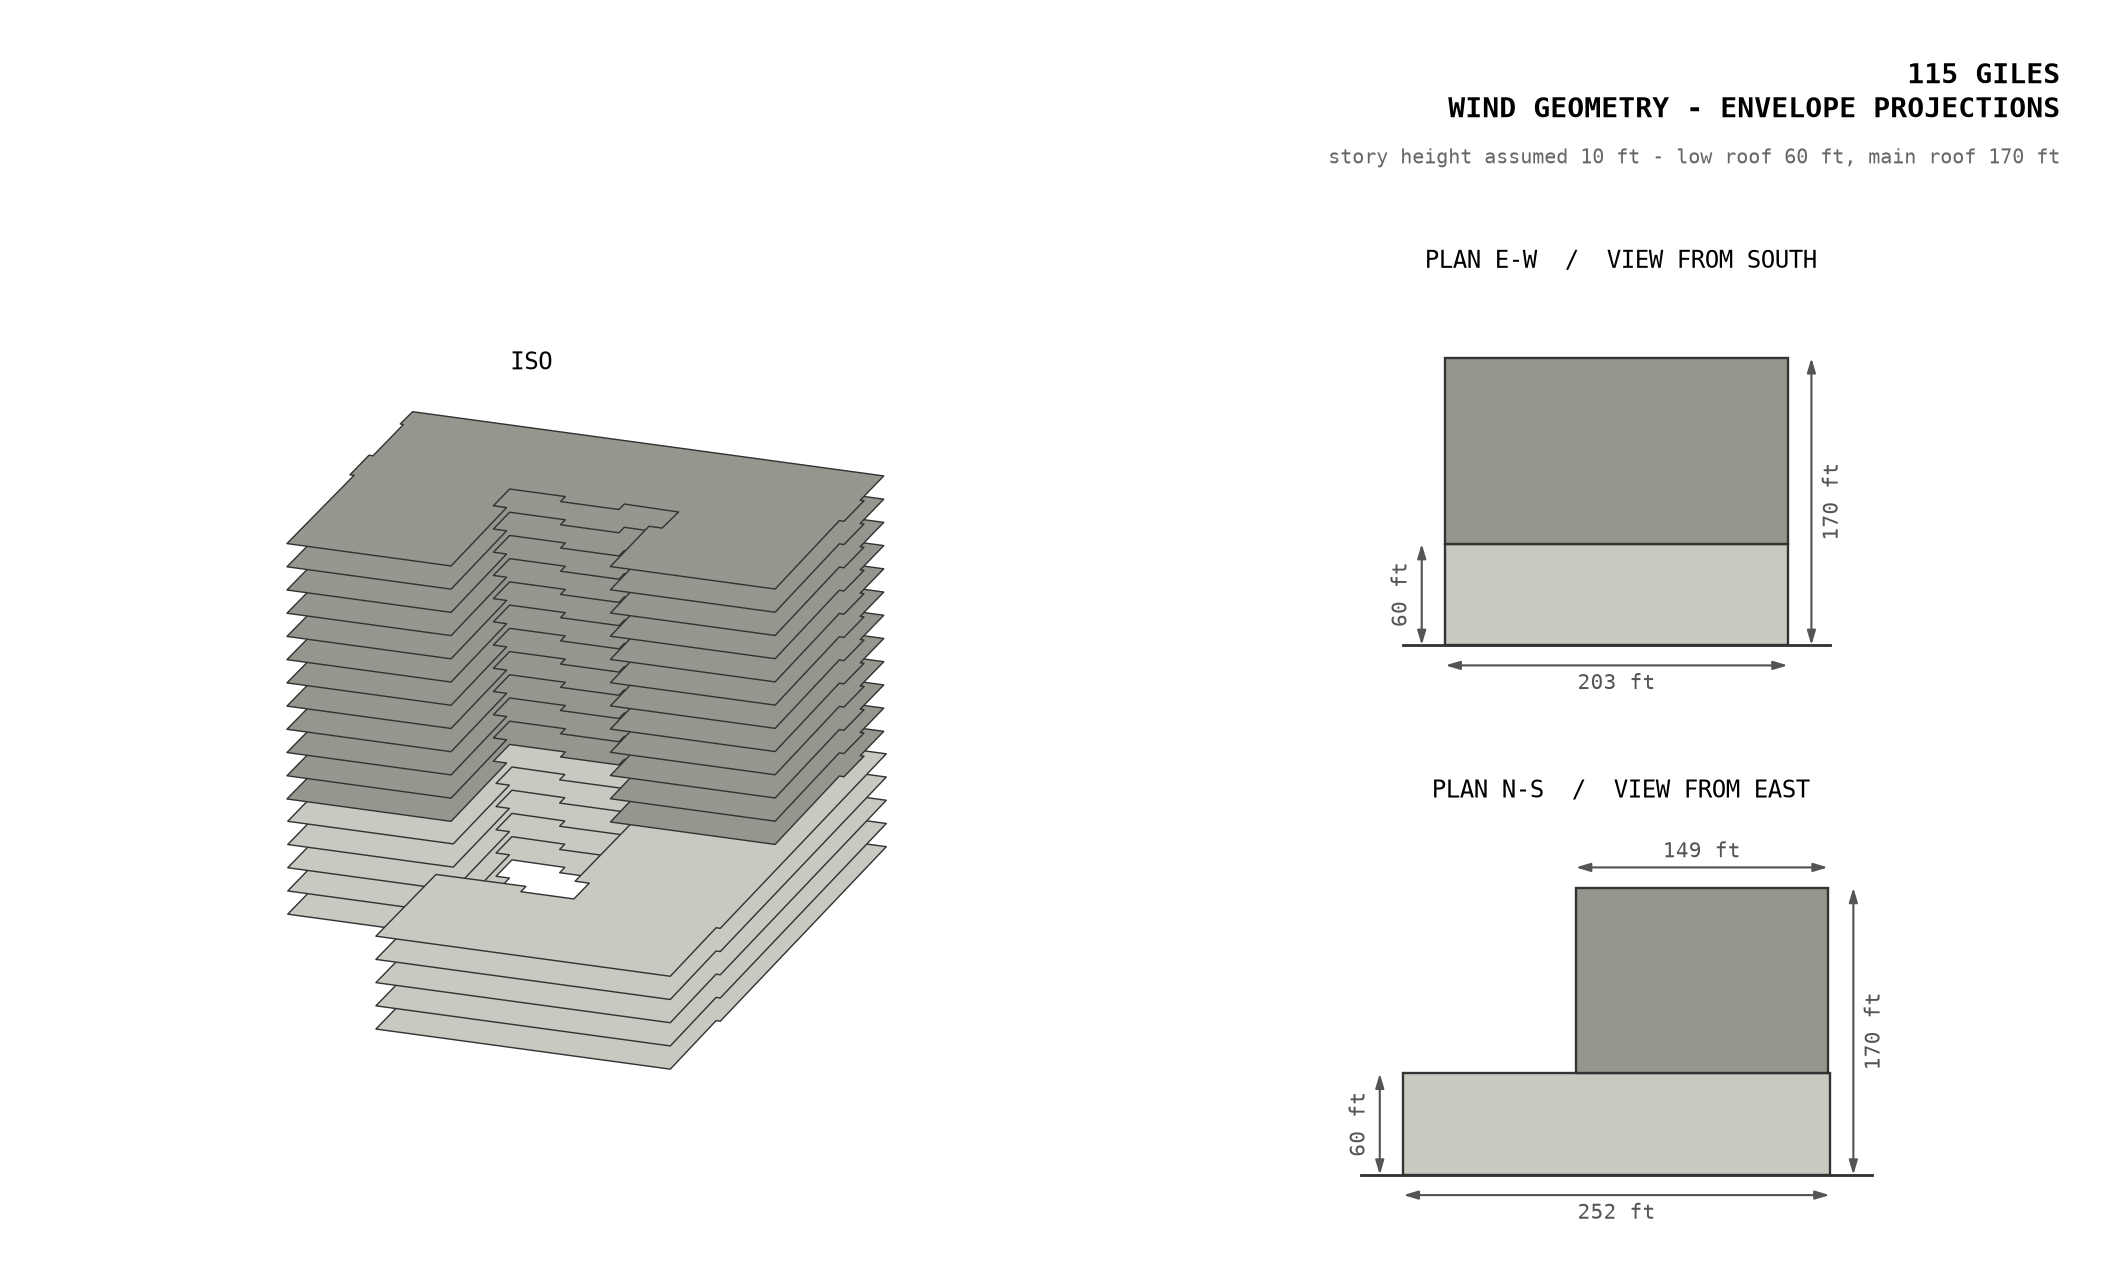
\includegraphics[width=\linewidth]{wind-geometry.png}

\subsection{Velocity Pressure}

\begin{equation}
q_z = 0.00256\,K_z K_{zt} K_e K_d V^2 = 0.00256(1.09)(1.0)(1.0)(0.85)(115)^2 = 31.4~\mathrm{psf}
\end{equation}
{\ttfamily\footnotesize \begin{tabular}{@{}ll@{}}
$K_z$ & exposure coefficient, Exp B at $z=h=170$ ft (ASCE 7-22) \\
$K_{zt}$ & topographic factor \\
$K_e$ & ground elevation factor \\
$K_d$ & directionality factor \\
$V$ & basic wind speed, 115 mph, Risk Cat II, Jersey City NJ \\
\end{tabular}}

\medskip
Adopt $q_z = 35$ psf uniform over full height ($\approx$11\% over $q_h$).

\subsection{Net Pressure (Windward + Leeward)}

\begin{equation}
p = q_z\,G\,(C_{p,ww} + |C_{p,lw}|) = 35(0.85)(0.8 + 0.5) = 38.7~\mathrm{psf}
\end{equation}
{\ttfamily\footnotesize \begin{tabular}{@{}ll@{}}
$G$ & gust-effect factor \\
$C_{p,ww}$ & windward wall pressure coefficient, $+0.8$ \\
$C_{p,lw}$ & leeward wall pressure coefficient, $-0.5$ ($L/B \le 1$; N-S wind $L/B \approx 1.25 \rightarrow -0.45$, use $-0.5$) \\
\end{tabular}}

\medskip
Adopt $p = 40$ psf net on projected area, both directions.

\subsection{Base Shear}

\begin{equation}
V_x = p\,A_x = 40\,(252 \cdot 60 + 149 \cdot 110)/1000 = \boxed{1{,}260~\mathrm{k}}
\end{equation}
\begin{equation}
V_y = p\,A_y = 40\,(203 \cdot 170)/1000 = \boxed{1{,}380~\mathrm{k}}
\end{equation}
{\ttfamily\footnotesize \begin{tabular}{@{}ll@{}}
$A_x$ & projected area for wind along X (E-W), N-S elevation profile \\
$A_y$ & projected area for wind along Y (N-S), E-W elevation profile \\
\end{tabular}}

\section{EQ}

\subsection{Geometry}

\noindent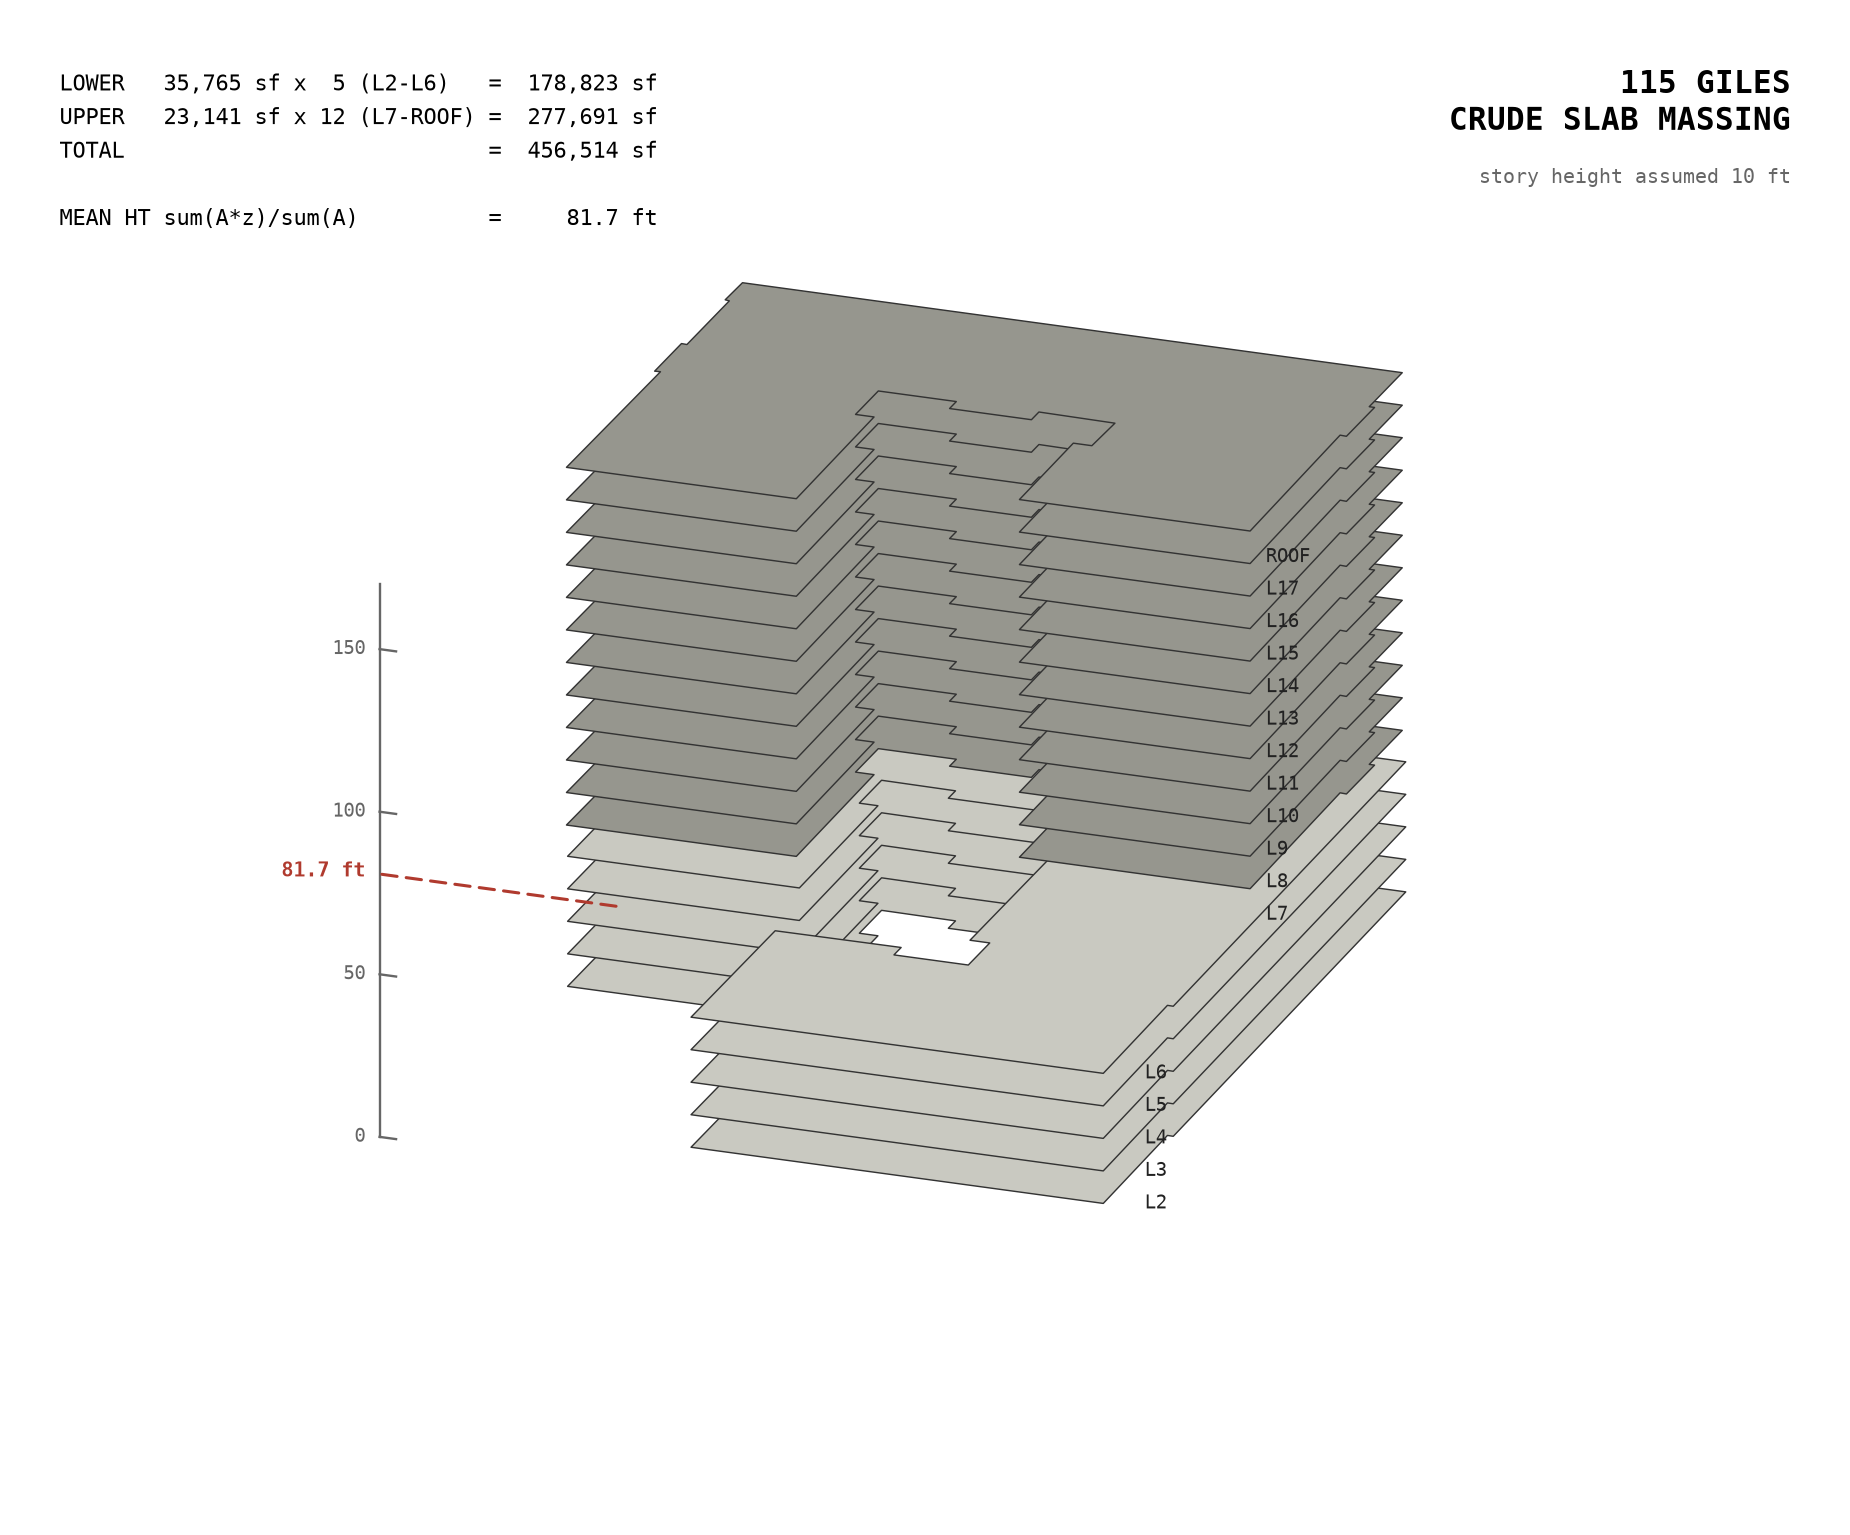
\includegraphics[width=\linewidth]{eq-massing-iso.png}

\subsection{Loads}

\begin{equation}
w = w_{slab} + w_{SDL} = 100 + 35 = 135~\mathrm{psf}
\end{equation}
{\ttfamily\footnotesize \begin{tabular}{@{}ll@{}}
$w_{slab}$ & 8 in slab self-weight, 100 psf, all floors \\
$w_{SDL}$ & superimposed dead load, 35 psf, all floors \\
\end{tabular}}

\begin{equation}
W = w \, \Sigma A = 0.135(456{,}514) = 61{,}629~\mathrm{k}
\end{equation}
{\ttfamily\footnotesize \begin{tabular}{@{}ll@{}}
$W$ & effective seismic weight \\
$\Sigma A$ & total slab area above base, per 2.1 \\
\end{tabular}}

\newpage
\subsection{Hazard / Site}

Case study: ASCE 7-16 site-coefficient chain vs ASCE 7-22 direct multi-period, both Site Class D assumed (no geotech).

\medskip
\noindent
\begin{minipage}[t]{0.48\linewidth}
\centering {\ttfamily\footnotesize\bfseries ASCE 7-16}
\begin{align*}
S_{MS} &= F_a S_S = 1.58(0.28) = 0.44 \\
S_{M1} &= F_v S_1 = 2.40(0.051) = 0.12 \\
S_{DS} &= \tfrac{2}{3} S_{MS} = 0.30 \\
S_{D1} &= \tfrac{2}{3} S_{M1} = 0.082
\end{align*}
\end{minipage}\hfill
\begin{minipage}[t]{0.48\linewidth}
\centering {\ttfamily\footnotesize\bfseries ASCE 7-22}
\begin{align*}
S_{MS} &= 0.30 \ \text{(tool, direct)} \\
S_{M1} &= 0.10 \ \text{(tool, direct)} \\
S_{DS} &= \tfrac{2}{3} S_{MS} = 0.20 \\
S_{D1} &= \tfrac{2}{3} S_{M1} = 0.067
\end{align*}
\end{minipage}

{\ttfamily\footnotesize \begin{tabular}{@{}ll@{}}
$S_S$, $S_1$ & mapped MCE$_R$ accelerations, 0.28 / 0.051 \\
$F_a$, $F_v$ & site coefficients (7-16 Tables 11.4-1/2) \\
$S_{MS}$, $S_{M1}$ & site-adjusted MCE$_R$; 7-22 values direct from ASCE 7 Hazard Tool \\
$S_{DS}$, $S_{D1}$ & design accelerations \\
\end{tabular}}

\medskip
Risk Cat II, $I_e = 1.0$. SDC B both cases.

\subsection{System / Period}

Ordinary reinforced concrete shear walls, bearing wall system, $R = 4$.

\begin{equation}
T_a = C_t h_n^x = 0.02(170)^{0.75} = 0.94~\mathrm{s}
\end{equation}
{\ttfamily\footnotesize \begin{tabular}{@{}ll@{}}
$R$ & response modification coefficient \\
$C_t$, $x$ & approximate-period coefficient / exponent, all other systems \\
$h_n$ & structural height above base, 170 ft \\
\end{tabular}}

\subsection{Base Shear (ELF)}

\begin{equation}
C_s = \frac{S_{DS}}{R/I_e} \qquad
C_{s,max} = \frac{S_{D1}}{T\,(R/I_e)} \qquad
C_{s,min} = 0.044\,S_{DS} I_e \ge 0.01 \qquad
V = C_s W
\end{equation}
{\ttfamily\footnotesize \begin{tabular}{@{}ll@{}}
$C_s$ & seismic response coefficient, bounded by $C_{s,max}$ / $C_{s,min}$ \\
$T$ & period used in direction considered, $T = T_a = 0.94$ s \\
\end{tabular}}

\medskip
\noindent
\begin{minipage}[t]{0.48\linewidth}
\centering {\ttfamily\footnotesize\bfseries ASCE 7-16}
\begin{align*}
C_s &= 0.30/4 = 0.075 \\
C_{s,max} &= \tfrac{0.082}{0.94(4)} = 0.0218 \ \leftarrow \\
C_{s,min} &= 0.044(0.30) = 0.0132 \\
V &= 0.0218(61{,}629) = \boxed{1{,}344~\mathrm{k}}
\end{align*}
\end{minipage}\hfill
\begin{minipage}[t]{0.48\linewidth}
\centering {\ttfamily\footnotesize\bfseries ASCE 7-22}
\begin{align*}
C_s &= 0.20/4 = 0.050 \\
C_{s,max} &= \tfrac{0.067}{0.94(4)} = 0.0178 \ \leftarrow \\
C_{s,min} &= 0.01~\text{(floor)} \\
V &= 0.0178(61{,}629) = \boxed{1{,}097~\mathrm{k}}
\end{align*}
\end{minipage}

\medskip
7-16 governs, $+23\%$. $C_{s,max}$ controls both cases.

\end{document}
